\documentclass[12pt,a4paper]{article}

 
\usepackage{xcolor}

\usepackage{tikz}
\usetikzlibrary{arrows.meta}


% Some colors I like. The first six are modified versions of colors from
% the Gnome Project "Tango" palette.
\definecolor{plum}{rgb}{0.36078, 0.20784, 0.4}
\definecolor{chameleon}{rgb}{0.30588, 0.60392, 0.023529}
\definecolor{cornflower}{rgb}{0.12549, 0.29020, 0.52941}
\definecolor{scarlet}{rgb}{0.8, 0, 0}
\definecolor{brick}{rgb}{0.64314, 0, 0}
\definecolor{sunrise}{rgb}{0.80784, 0.36078, 0}
\definecolor{lightblue}{rgb}{0.15,0.35,0.75}
\definecolor{carolina}{RGB}{153, 186, 221}

% A custom arrowhead for use on x, y, z axes
\tikzstyle{axisarrow} = [-{Latex[inset=0pt,length=5pt]}]

\begin{document}

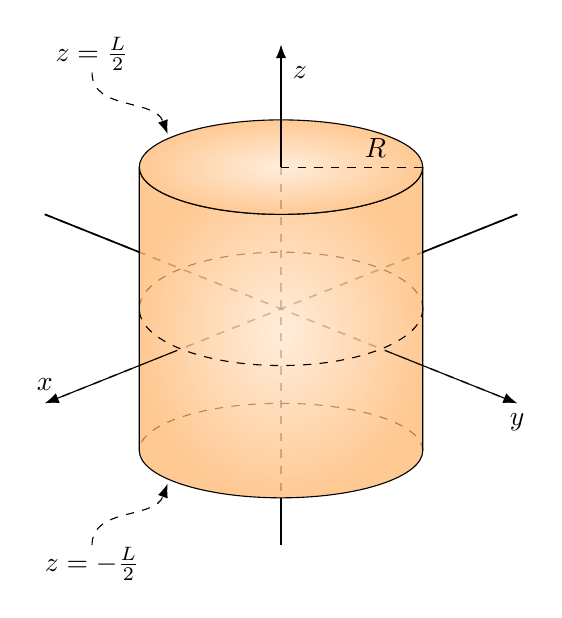
\begin{tikzpicture}[scale=1.2]
	% Draw the grid.
%	\draw [cornflower!20,step=0.25,thin] (-3,-3) grid (3,3);
%	\draw [cornflower!40,step=1.0,thin] (-3,-3) grid (3,3);

	\draw[semithick,opacity=0.6,dashed] (0,1.5) -- (0,-2.5);
	\draw[semithick] (0,-2) -- (0,-2.5);
	\draw[semithick,axisarrow,dashed,opacity=0.6] (-2.5,1) -- (2.5,-1);
	\draw[semithick] (-2.5,1) -- (-1.5,0.6);
	\draw[semithick,axisarrow,dashed,opacity=0.6] (2.5,1) -- (-2.5,-1);
	\draw[semithick] (1.5,0.6) -- (2.5,1);

    \draw[dashed] (1.5,0) arc (0:180:1.5cm and 0.6cm);

    \draw[dashed] (1.5,-1.5) arc (0:180:1.5cm and 0.5cm);
	\shade[shading=radial, inner color=orange!20!white, outer color=orange!60!white, opacity=0.70] (1.5,1.5) -- (1.5,-1.5) arc (360:180:1.5cm and 0.5cm) -- (-1.5,1.5) arc (180:360:1.5cm and 0.5cm) ;
	\draw[] (1.5,1.5) -- (1.5,-1.5) arc (360:180:1.5cm and 0.5cm) -- (-1.5,1.5) arc (180:360:1.5cm and 0.5cm) ;
 
  \draw[dashed] (1.5,0) arc (360:180:1.5cm and 0.6cm);

  \shade[shading=radial, inner color=orange!20!white, outer color=orange!60!white, opacity=0.70] (1.5,1.5) arc (0:360:1.5cm and 0.5cm); 
  \draw (1.5,1.5) arc (0:360:1.5cm and 0.5cm);


  \draw [dashed] (0,1.5)--(1.5,1.5);
	\node at (1.0,1.7) {$R$};

	\draw[semithick,axisarrow] (0,1.5) -- (0,2.8);
	\node at (.2,2.5) {$z$};
	\draw[axisarrow] (1.1,-.44) -- (2.5,-1);
	\node at (2.5,-1.2) {$y$};
	\draw[axisarrow] (-1.1,-.44) -- (-2.5,-1);
	\node at (-2.5,-0.8) {$x$};
	
	\draw[dashed] (-2,-2.5) edge[out=90,in=250,axisarrow] (-1.2,-1.85);
	\node[] at (-2,-2.7) {$z=-\frac{L}{2}$};

	\draw[dashed] (-2,2.5) edge[out=270,in=110,axisarrow] (-1.2,1.85);
	\node[] at (-2,2.7) {$z=\frac{L}{2}$};

\end{tikzpicture}	

\end{document}